\documentclass[a4paper,12pt]{report}
\usepackage{graphicx}
\usepackage{array}
\graphicspath{{./images/}}

\begin{document}
	
	\begin{titlepage}
		\begin{center}
			
\includegraphics{ankara_bilim.png}
		\end{center}
		\vspace{1cm}
		\begin{center}
			\LARGE
			\textbf{SENG 244 - Object Oriented Software Engineering}
		\end{center}
		\vspace{1cm}
		\begin{center}
			\Large
			\textbf{Software Design Document}
		\end{center}
		\vspace{1cm}
		\begin{center}
			\Large
			\textbf{Non Governmental Organization - Aid Operations Management System}
		\end{center}
		\vspace{2cm}
		\begin{center}
			\large
			\textbf{BETG-4}
		\end{center}
		\vspace{1cm}
		\begin{center}
			\large
			Bora Eskin - 210201021\\
			Eren Demir Özalban - 220201031\\
			Talha Fatih Bülbül - 220204007\\
			Gürkan Köleoğlu - 200204043
		\end{center}
	\end{titlepage}
	
	\tableofcontents
	
	\chapter{Introduction}
		\section{Purpose of System}
  			\paragraph{}The NGO Aid Operations Management System (NGO-AOMSYS) is designed to streamline the process of managing aid provisions for Non-Governmental Organizations (NGOs).
     			\paragraph{}The system aims to efficiently allocate and distribute aid, both in-kind and in-cash, to indigent individuals and households in need.
	  		\paragraph{}By providing a platform for donors to contribute, volunteers to engage, and aid recipients to apply for assistance, NGO-AOMSYS aims to improve the overall effectiveness and transparency of aid operations.
		\section{Design Goals}
  			\paragraph{}Efficiency: Automate the process of donation collection, volunteer registration, and aid distribution to reduce manual effort and improve response time.
     			\paragraph{}Transparency: Provide donors, volunteers, and aid recipients with visibility into the aid allocation process, including tracking their contributions and assistance requests.
			\paragraph{}Scalability: Accommodate a growing number of users, donations, and aid requests without compromising system performance.
   			\paragraph{}Accessibility: Ensure that the system is user-friendly and accessible to individuals with varying levels of technical expertise.
		\section{Definitions, Acronyms and Abbreviations}
  			\paragraph{}Donor: An individual or organization that contributes funds or materials to the NGO-AOMSYS system.
     			\paragraph{}Volunteer: An individual who offers their time and services to support aid operations.
			\paragraph{}Indigent: Individuals or households in need of aid assistance.
   			\paragraph{}Geographic Information System (GIS): A system designed to capture, store, manipulate, analyze, manage, and present spatial or geographic data.
      			\paragraph{}In-kind: Non-monetary contributions such as goods, services, or materials.
	 		\paragraph{}In-cash: Monetary contributions.
    			\paragraph{}Work Breakdown Structure (WBS): A hierarchical decomposition of the total scope of work to be carried out by the project team.
		\section{References}
  			\paragraph{} NGO Coordination Resource Center. (2024). "Title." Access Date: [29/04/2024], Access Address: [https://ngocoordination.org/en/library/types/manual-toolkits-and-guidance].
		\section{Overview}
  			\paragraph{}This document provides a detailed description of the NGO Aid Operations Management System (NGO-AOMSYS) software design. It outlines the purpose of the system, design goals, definitions, acronyms, and abbreviations used. The document also includes a reference section listing sources of information. The subsequent sections of the document will delve into the system's architecture, functionality, user interface, database design, and other key aspects.
	\chapter{Current Software Architecture}
		-
	\chapter{Proposed Software Architecture}
		\section{Overview}
			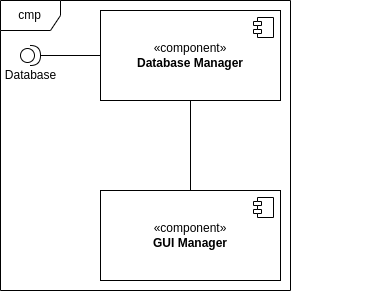
\includegraphics{component_diagram.png}
			\paragraph{}The product being developed is mainly made up of two components. The Database Manager and GUI Manager. Database Manager can be considered as the entire system of backend and GUI Manager the entire system of frontend. Database Manager, as the name implies, is responsible for managing the database. While the GUI Manager handles what to be shown to the user. 
		\section{Subsystem Decomposition}
			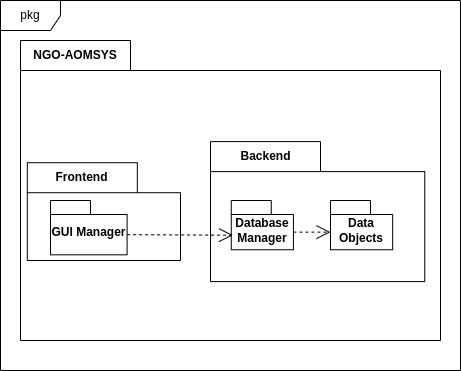
\includegraphics{subsystem_decomposition_diagram.png}
			\paragraph{NGO-AOMSYS} This is the system being developed in its entirety, just a formality.
			\paragraph{Frontend} This is the frontend part of the program.
			\paragraph{Backend} This is the backend part of the program.
			\paragraph{GUI Manager} This part of the software is used to communicate with the user through a graphical interface. It depends on Database Manager for the reason of retrieving needed information that needs to presented to the user.
			\paragraph{Database Manager} This part of the software is used to communicate between data objects and the database. It depends on the Data Objects.
			\paragraph{Data Objects} This part of the software is used to structure data in an organized manner into objects.
		\section{Hardware/Software Mapping}
			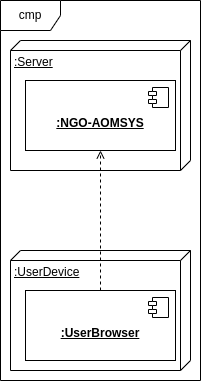
\includegraphics{hardware_software_mapping.png}
		\section{Persistent Data Management}
			\paragraph{} All data is managed by an instance of class DatabaseManager in program. The instance of DatabaseManager communicates with an actual database to accomplish persistent data. DatabaseManager serves as a center of all data management.
		\section{Access Control and Security}
			\begin{tabular}[array]{|m{78pt}|m{78pt}|m{78pt}|m{78pt}|m{78pt}|}%78=textwidth/5, textwidth=390pt
				\hline
				&Donor&Operation\newline Coordinator&System\newline Administrator&Volunteer\\
				\hline
				Donation\newline&RW&R&RW&R\\
				\hline
				Shipment\newline Request&RW&RW&RW&R\\
				\hline
				Aid\newline Registration&-&RW&RW&R\\
				\hline
				Aid\newline Operation&-&RW&RW&R\\
				\hline
				Personal\newline Profile&-&R&RW&RW\\
				\hline
			\end{tabular}
			\paragraph{} 
		\section{Boundary Conditions}
			\paragraph{} The startup only consists of DatabaseManager loading data as their respective class into memory by communicating with the database itself.
			\paragraph{} There are no other notably different processes in other areas. 
		\section{Subsystem Services Glossary}
			\paragraph{Database Manager} It communicates the data with GUI Manager and database using data objects, and thus it is a service for both.
			\paragraph{GUI Manager} It communicates the data with GUI Manager and user, and thus it is a service for both.
	\chapter{Object Design}
		\section{Object Design Trade-Offs}
			\paragraph{} The only consideration for the design of the objects was ease of implementation due to time constraints.
			\paragraph{} The design choice depends on centralization using only two classes to manage the entire system as frontend and backend.
			\paragraph{} The naming convention for the object identifiers is camel case with uppercase letter at the start of the identifier.
		\section{Interface Documentation Guidelines}
			\begin{itemize}
				\item Classes are named using camel case with starting uppercase letter.
				\item Methods are named using snake case.
				\item Method parameters are named using snake case.
				\item All objects being developed as a part of the system are separate files.
				\item Errors are returned as return values.
			\end{itemize} 
		\vspace{100cm}
		\section{Packages}
		
		\textbf{Frontend:}
		
			\paragraph{  }  The main reason of the frontend is accebility and usability of the software. It's uses niceGui library which is a phyton script for web. İts make it possible to used by regular human knowledge. It's satisfices the tasks of registration, managing donations and system admin work. It's supports different types of users. It's set up in a way that separates tasks by user role.  \\
			
				\textbf{Backend:}
					\paragraph{ } The backend is the core of the whole system. İts manages the whole charity application. It abstracts the backend storage and management of various entities and operations. İt makes sure that entities correctly created, retrieved, updated, and deleted, facilitating. 
				
		
		\section{Class Interfaces Glossary}
		
			\textbf{Frontend:}
			\underline{GuiManager}
				\begin{itemize}
				\item @ui.page("/"),
				 The main page of the app. It  sends users  to the login page.
				 	\item@ui.page("/login")
				 	This page lets users log in by entering their username and password. If the details are match, it directs them to a page to their role. If does not match with any, it gives a error message.
				 	\item@ui.page("/register")
				 	It's for the registration of the new user. They need to fill out their details like username, password, and email, and choose their role. Once done, it sends them to the login page.
				 	\item@ui.page("/manage-account")
				 	This lets users change their password. It checks if the old password is correct before updating it.
				 		\item@ui.page("/aid-registration-form")
				 	İn order to ask help user can fill the form. The form asks for  many kids they have, what their income is, and what kind of help they need and household members.
				 	\item@ui.page("/donor-menu")
				 	This page is for donors to look at and manage their donations and requests for shipments. They can also start new donations and shipment requests here.
				 		\item@ui.page("/volunteer-menu")
				 		This menu lets volunteers look at their aid operations. It helps them get more involved and be more effective in the organization.
				 		\item@ui.page("/operation-coordinator-menu")
				 		 this page is for the coordinators, it manage  collecting items, shipping, and setting up public events. It makes it visible operations and lets them add new ones.
				 		\item@ui.page("/system-administrator-menu")
				 		 The system for to admins to manage the app. They can see the user accounts check and  manage them. 
				 	
				 	
				 	
				 
			\end{itemize}
				\textbf{Backend:}
			\underline{DataBase Objects} \\
			
			\textit{AidOperation Class:} 
			\begin{itemize}
			
				\item getAddress: Gets where the operation's happening.
				\item setAddress: Writes in where the operation's gonna be.
				\item getID: Fetches the operation’s unique number.
				\item getOperationCoordinatorID: Gets the ID for the person running the show.
				\item setOperationCoordinatorID: Sets the ID for the boss of the operation.
				
				
				
				
			\end{itemize}
			
				\textit{AidRegistration Class:} 
			\begin{itemize}
				
		\item	init: Sets up a new aid request with all the starting details like who needs help and how much money they make.
		\item	get/setNumberOfChildren: Checks or sets how many kids are in the family.
		\item	get/setMonthlyIncome: Looks at or updates how much money the family makes a month.
		\item get/setAddress: Gets or changes the family's address.
			get/setMonthlyExpenditures: Checks or changes how much the family spends a month.
		\item	get/setNatureOfSupportNeeded: Finds out or updates what kind of help they need.
	        \item add/removeHouseholdMember: Adds or removes people from the household in the system.
			getID: Gives back the unique number for this aid request.
			
		\end{itemize}
				\textit{CollectItemsOperation Class:} 
				\begin{itemize}
					
				 \item	init: Starts an operation specifically for collecting items, keeping track of where stuff needs to go.
				 \item	get/setDestinationAddress: Gets or sets where the collected items need to end up.
					
				\end{itemize}
				
				\textit{Donation Class:} 
				\begin{itemize}
					
				\item	init: Kicks off a new donation record.
				\item	get/setTypeOfDonation: Figures out or sets what kind of donation it is.
				\item	get/setAmount: Checks or updates how much was given.
				\item	get/setArea: Looks at or changes where the donation is for.
				\item	get/setDonorID: Gets or sets who gave the donation.
				\item	get/setShipmentRequestID: Connects the donation to a shipment or changes that connection.
					
				\end{itemize}
			
				\textit{Donor Class:} 
			\begin{itemize}
				
		\item	init: Starts up a donor's account.
		\item	getDonations/getShipmentRequests: Lists all the donations or shipment requests they've made.
		\item	add/removeDonation: Adds or pulls a donation from their record.
		\item	add/removeShipmentRequest: Starts or deletes a shipment request they've asked for.
		\item	getDonationByID/getShipmentRequestByID: Finds a specific donation or shipment request by its ID.
				
			\end{itemize}
				\textit{IndigentPerson Class:} 
			\begin{itemize}
				\item	init: Sets up the basic info for someone in need.
				\item	get/setName: Gets or sets their name.
				\item	get/setSurname: Checks or updates their last name.
				\item	get/setEmploymentStatus: Looks at or changes their job situation.
				\item	get/setEducationalStatus: Checks or updates their school status.
				\item	get/setAge: Finds out or sets how old they are.
			\end{itemize}
			
				\textit{OperationCoordinator Class:} 
			\begin{itemize}
			\item	init: Sets up a user who manages operations.
			\item	getAidOperations: Lists all the operations they’re handling.
			\item	add/removeAidOperation: Adds or removes an operation from their list.
			\item	getAidOperationByID: Finds an operation by its ID.
			
			\end{itemize}
			
			
			
			\textit{PersonalProfile Class:} 
			\begin{itemize}
			\item	init: Starts a new profile with all personal details set to default.
			\item	get/setProfession: Looks at or updates their job.
			\item	get/setAverageAnnualIncome: Checks or changes how much they make a year.
			\item	get/setSelectedRegion: Finds out or sets where they’re based.
			\item	get/setTransportationSupport: Checks or changes if they have transport help.
			\item	get/setAvailability: Sees or updates when they’re available.
			\item	get/setAccepted: Checks or changes if their profile is okayed.
			\item	getIsPending: Sees if their profile is still waiting to be checked.
			\item	get/setVolunteerID: Gets or sets their volunteer ID.
		\end{itemize}
				
					\textit{PublicEventOperation Class:} 
				\begin{itemize}
					\item	nit: Starts planning a public event.
					\item	get/setEventName: Looks at or sets the name of the event.
					\item	ShipItemsOperation Class
					
					\item	init: Kicks off an operation to send items somewhere.
					\item	get/setDestinationAddress: Finds out or sets where the items need to go.
					
			\end{itemize}
			
			
			\textit{ShipmentRequest Class:} 
			\begin{itemize}
		\item	init: Begins a new request for shipping something.
		\item	get/setAddress: Checks or updates where the shipment's going.
		\item	isSelfShipped/isShippedByNGO: Checks if it’s being sent by the donor themselves or an NGO.
		\item	setSelfShipped/setShippedByNGO: Picks if the donor or an NGO is doing the shipping.
		\item	getID/getDonationID/getDonorID: Gets the unique ID for the request, the donation connected to it, or who's sending it.
				
			\end{itemize}
			
			
			\textit{User Class:} 
			\begin{itemize}
				\item	init: Sets up a new user.
				\item	get/setUsername: Gets or changes their username.
				\item	isPasswordCorrect: Checks if their password is right.
				\item	get/setName: Sees or changes their first name.
				\item	get/setSurname: Checks or updates their last name.
				\item	setEmail: Changes their email.
				\item	getID: Gets their unique user ID.
			\end{itemize}
			
			
			\textit{Volunteer Class:} 
			\begin{itemize}
		\item	init: Starts a new volunteer profile.
		\item	get/setPersonalProfile: Looks at or updates their personal profile details.
			\end{itemize}
			
				\underline{DataBase Manager} \\
			
			
			\begin{itemize}
				\item	Constructor : Initializes lists to manage volunteers, coordinators, administrators, donors, and various operations and requests like donations, shipment requests, and aid operations.
				
				\item	getDonorByID(self, input): Returns a Donor object matched by ID.
				\item	getVolunteerByID(self, input): Retrieves a Volunteer by looking for a match by the ID.
				\item	getOperationCoordinatorByID(self, input): Get  OperationCoordinator by ID.
				\item	getSystemAdministratorByID(self, input): Get a SystemAdministrator by ID.
				\item	getUserByID(self, input): Get any user  by ID.
				\item	getDonationByID(self, input): Gets a Donation object by ID.
				\item	getShipmentRequestByID(self, input): Gets a ShipmentRequest by ID.
				\item	getAidRegistrationByID(self, input): Gets an AidRegistration information by ID.
				\item	getPersonalProfileByID(self, input): Gets a PersonalProfile by ID.
				\item	getAidOperationByID(self, input): Gets any type of aid operation (ship items, collect items, public event) by ID.
				
				\item	getDonations(self): Returns all recorded donations.
				\item	getShipmentRequests(self): Lists all shipment requests.
				\item	getAidRegistrations(self): Returns all aid registrations.
				\item	getAidOperations(self): Aggregates all types of aid operations.
				\item	getPersonalProfiles(self): Lists all personal profiles.
				\item	getUsers(self): Consolidates all user types into a single list.
				\item	getVolunteers(self): Returns all volunteers.
				\item	getOperationCoordinators(self): Lists all operation coordinators.
				\item	getSystemsAdministrators(self): Returns all system administrators.
				\item	getDonors(self): Lists all donors.
			
				\item	addDonor(self, ...): Adds a new donor to the system.
				\item	addOperationCoordinator(self, ...): Registers a new operation coordinator.
				\item	addSystemAdministrator(self, ...): Adds a new system administrator.
				\item	addVolunteer(self, ...): Registers a new volunteer.
				\item	addDonation(self, ...): Records a new donation.
				\item	addShipmentRequest(self, ...): Adds a new shipment request.
				\item	addAidRegistration(self, ...): Registers a new aid request.
				\item	makeIndigentPerson(self, ...): Creates a new indigent person profile.
				\item	addPersonalProfile(self, ...): Adds a new personal profile for a volunteer.
				\item	addShipItemsOperation(self, ...): Adds a new ship items operation.
				\item	addCollectItemsOperation(self, ...): Adds a new collect items operation.
				\item	addPublicEventOperation(self, ...): Registers a new public event operation.
				
				\item	removeDonor(self, ...): Removes a donor.
				\item	removeOperationCoordinator(self, ...): Removes an operation coordinator.
				\item	removeSystemAdministrator(self, ...): Removes a system administrator.
				\item	removeVolunteer(self, ...): Removes a volunteer and their associated profile.
				\item	removeDonation(self, ...): Deletes a donation.
				\item	removeShipmentRequest(self, ...): Deletes a shipment request.
				\item	removeAidRegistration(self, ...): Deletes an aid registration.
				\item	removePersonalProfile(self, ...): Deletes a personal profile.
				\item	removeAidOperation(self, ...): Removes an aid operation.
				\item	removeUser(self, ...): Removes a user from the system.
			
			\end{itemize}
			
		
\end{document}
